% kappa.tex
% ======================================================================

% Base class and packages
\documentclass{article}
\usepackage{amsmath}
\usepackage{bm}
\usepackage{lineno}
\usepackage{natbib}
\usepackage[onehalfspacing]{setspace}
\usepackage{physics}
\usepackage[colorlinks, citecolor=blue]{hyperref}
\usepackage[sort]{cleveref}  % needs to be loaded after hyperref
\usepackage{graphicx}
\graphicspath{{figures/}}

% Move floats to the end
\usepackage[nolists]{endfloat}
\renewcommand{\efloatseparator}{\mbox{}}

% Copernicus-style internal references
\crefname{chapter}{Chap.}{Chaps.}
\crefname{equation}{Eq.}{Eqs.}
\crefname{figure}{Fig.}{Figs.}
\crefname{section}{Sect.}{Sects.}
\crefname{table}{Table}{Tables}

% My commands
%\newcommand{\note}[1]{\textbf{[NOTE: #1]}}
\newcommand{\todo}[1]{\emph{[\textbf{Todo:} #1]}}
\newcommand{\mref}[0]{\textbf{[ref.]}}

% Vectors and tensors
\newcommand{\vect}[1]{\va*{#1}} % bold arrow vectors
\newcommand{\tens}[1]{\vb*{#1}} % bold tensors

% Differential operators
\renewcommand{\div}[1]{\mathrm{div}\,#1}            % divergence
\renewcommand{\grad}[1]{\vect{\mathrm{grad}}\,#1}   % gradient
\newcommand{\tdiv}[1]{\vect{\mathrm{div}}\,#1}      % tensor divergence
\newcommand{\tgrad}[1]{\tens{\mathrm{grad}}\,#1}    % tensor gradient
\newcommand{\matdv}[1]{\pdv{#1}{t}+\vect{v}\cdot\grad{}\,#1}  % material dv.

% Common notations
\newcommand{\doteps}[0]{\dot{\epsilon}} % epsilon dot
\newcommand{\IDT}[0]{\tens{\delta}}     % Identity tensor
\newcommand{\CST}[0]{\tens{\sigma}}     % Cauchy stress tensor
\newcommand{\DST}[0]{\tens{\tau}}       % deviatoric stress tensor
\newcommand{\SRT}[0]{\tens{\doteps}}    % strain-rate tensor
\newcommand{\vv}[0]{\vect{v}}           % velocity vector
\newcommand{\vsia}[0]{\vv_{\mathrm{SIA}}}   % SIA velocity
\newcommand{\vssa}[0]{\vv_{\mathrm{SSA}}}   % SSA velocity
\newcommand{\PDD}[0]{\mathrm{PDD}}
\newcommand{\sPDD}[0]{\sigma_{\mathrm{PDD}}}

% Common units
\newcommand{\e}[1]{\ensuremath{\times 10^{#1}}}
\newcommand{\chem}[1]{\ensuremath{\mathrm{#1}}}
\newcommand{\unit}[1]{\ensuremath{\mathrm{#1}}}
\newcommand{\degree}[0]{\ensuremath{^{\circ}}}
\newcommand{\degC}[0]{\unit{{\degree}C}}

% Papers of the thesis
\newcommand{\CCLI}[0]{Paper~I}      % Cordillera climate
\newcommand{\PSDV}[0]{Paper~II}     % PDD SD variability
\newcommand{\PSDP}[0]{Paper~III}    % PDD SD parametrisation
\newcommand{\CCYC}[0]{Paper~IV}     % Cordillera cycle

% Text label over graphics
% from http://tex.stackexchange.com/questions/128844/put-subfigure-labels-
% inside-figures-using-subfig-package
\newcommand{\subgraphics}[3][,]{%
  \setbox1=\hbox{\includegraphics[#1]{#3}}% Store image in box
  \leavevmode\rlap{\usebox1}% Print image
  \rlap{\hspace*{0.25em}
        \raisebox{\dimexpr\ht1-3ex}{\textbf{(#2)}}}% Print label
  \phantom{\usebox1}% Insert appropriate spacing
}

% Finally to not include graphics
%\renewcommand{\includegraphics}[2][,]{}
%\renewcommand{\subgraphics}[3][,]{}

% Document properties
\title{Numerical simulation of the Cordilleran ice sheet \\
       through the last glacial cycle}
\author{Julien Seguinot}

% ======================================================================
\begin{document}
% ======================================================================

\maketitle
\linenumbers
\tableofcontents

% ======================================================================
\section{Introduction}
% ======================================================================

In our daily lives, we most commonly experience ice as the small, solid cubes
that crackle on contact with refreshing liquids. Yet, at geological
time-scales, and under high stresses, ice behaves in a much different fashion.
In the cold and mountainous regions of the globe, ice accumulates under the
action of cumulative snowfall, until it reaches a critical thickness, and
deforms under its own weight to flow downhill (\cref{fig:glacier-mechanics}).
Glaciers, these bodies of moving ice, flow by a combination of water-induced
sliding at the base \citep{Saussure.1796}, and visco-plastic deformation within
the ice body \citep{Forbes.1846b}.

As ice flows and glides on its bed, it transports rock debris and erode the
landscape, thence leaving geomorphological traces of its former presence
(\cref{fig:glaciation-indicators}). In many parts of the world, montane people
and early explorers have since long learned to read these traces, and to
understand that glaciers had once been more extensive than today. With the
advent of the glacial theory, birthed the idea that, under colder temperatures
than today, expansive \emph{ice sheets} had once covered much of Europe and
North America \citep{Agassiz.1840}.

However, the glacial theory did not gain much belief until the exploration and
discovery of the two present-day ice sheets on Earth, the Greenland and
Antarctic ice sheets, provided a modern analogue for the proposed European and
North American ice sheets. The first traverse of the Greenland was performed by
Nansen in 1888, while Amundsen reached the south pole in 1911. Meanwhile, in
the European Alps, it was then discovered from observations of the glacial
landscape, that there had not been only one, but at least four, glacial periods
\citep{Penck.Bruckner.1909}.

More recently, palaeo-climate records extracted from deep-sea sediments have
provided a much more detailed picture of the Earth environmental history
\citep[e.g.,][]{Emiliani.1955, Shackleton.Opdyke.1973}, thus indicating neither
one, nor four, but rather tens of glacial cycles. During the last million
years, glacial and interglacial cycles have succeeded each other with a
100\,kyr periodicity \citep{Hays.etal.1976}. In the present thesis, we focus on
the most recent of these cycles: \emph{the last glacial cycle}
(\cref{fig:paleo-timeseries})

% ice volume 26.07 + 2.93 = 29.00
% meters sea-level 58.3 + 0.70 = 59.0
Together, the Greenland and Antarctic ice sheets currently host most glacial
ice on the planet, corresponding to 59~meters of potential sea-level rise
\citep{Bamber.etal.2001, Fretwell.etal.2013}. At the apogee of the last glacial
cycle, the last glacial maximum, sea-level was 120 to 135\,m lower than today
\citep{Clark.Mix.2002}, implying an additional, double amount of ice stored in
ice sheets and glaciers on land. Systematic mapping and compilation of glacial
landforms from all continents permitted reconstructions of this former ice
cover \citep{Ehlers.Gibbard.2007}, indicating that ice volume
was repartitioned between more extensive Greenland and Antarctic ice sheets,
the Scandinavian and Barents-Kara ice sheets in the Eurasian arctic, and the
Innuitian, Laurentide and \emph{Cordilleran} ice sheets over North America
(\cref{fig:paleo-glaciation}).

Nevertheless, the landscape record is sparse in time and most often spatially
incomplete. Palaeo-ice sheets did not leave a systematic record of their
passage, and much of the evidence has been overridden by subsequent glacier
re-advances and other geomorphological processes \citep{Kleman.1994}.
Therefore, geomorphological reconstructions of former glacier extent require a
substantial amount of interpretation. This is where numerical models,
incorporating the processes of glacier sliding \citep[e.g.,][]{Weertman.1957}
and deformation \citep[e.g.,][]{Nye.1953} observed on modern glaciers, can help.
Although these models alone contain too many uncertainties to reproduce
accurate picture of past glacial cycles \citep[e.g.,][]{Hebeler.etal.2008},
they can be calibrated against geological data where they exist, while
allowing a physics-based, quantitative reconstruction where they do not.

\begin{figure}
  \centering
  \makebox[0pt]{
    \subgraphics{a}{photo-glacier-crevasses}
    \hspace{1cm}
    \subgraphics{b}{photo-glacier-susitna}
    \hspace{1cm}
    \subgraphics{c}{photo-glacier-fold}
  }
  \caption{Illustration of various glacier ice behaviours.
           \textbf{(a)} Surface crevasses formed by ice flow over a hidden
           bedrock knob. Glacier Blanc, French Alps, 2004.
           \textbf{(b)} Medial moraines illustrating downhill ice flow on
           Susitna Glacier, Alaska Range, by Austin Post, 1970
           \citep{NSIDC.2009}.
           \textbf{(c)} Mountain glacier calving into a small lake, revealing a
           folded structure formed by deformed debris layers in the ice.
           Glacier d'Arsine, French Alps, 2004.}
  \label{fig:glacier-mechanics}
\end{figure}

% Alternative code using subcaption package
%\usepackage{subcaption}
%\begin{figure}
%  \centering
%  \makebox[0pt]{
%    \begin{subfigure}[t]{80mm}
%        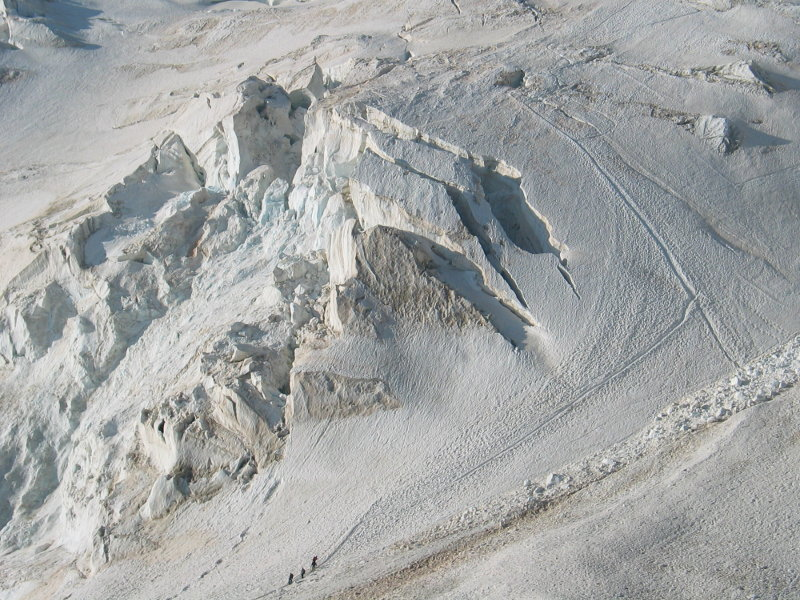
\includegraphics{photo-glacier-crevasses}
%        \caption{Subcaption a.}
%        \label{fig:1a}
%    \end{subfigure}
%    \hspace{10mm}
%    \begin{subfigure}[t]{80mm}
%        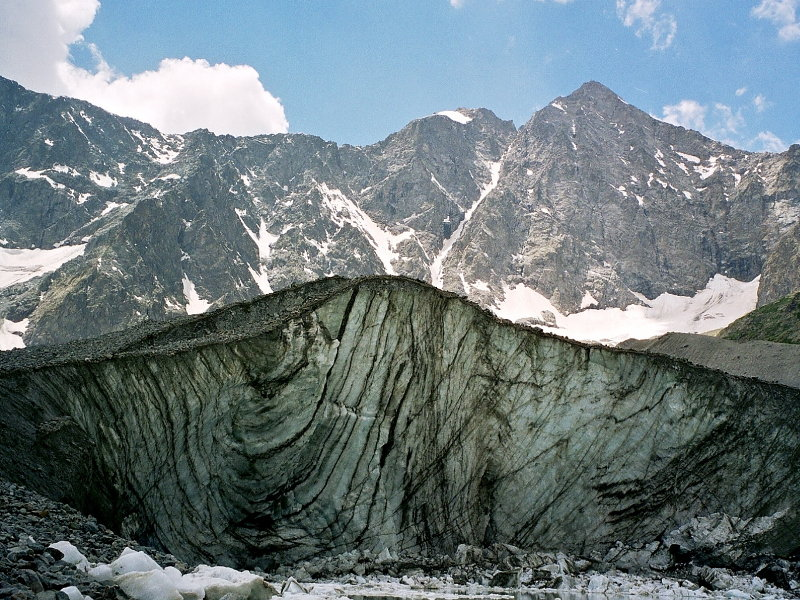
\includegraphics{photo-glacier-fold}
%        \caption{Subcaption b.}
%        \label{fig:1b}
%    \end{subfigure}
%  }
%  \caption{Global caption.}
%  \label{fig:1}
%\end{figure}

\begin{figure}
  \centering
  \makebox[0pt]{
    \subgraphics{a}{photo-glacial-valley}
    \hspace{1cm}
    \subgraphics{b}{photo-erratic-boulder}
    \hspace{1cm}
    \subgraphics{c}{photo-melt-channels}
  }
  \caption{Different indicators of past glaciation.
           \textbf{(a)} Glacial valley, exhibiting a broad, U-shaped profile
           characteristic of erosion by glaciers.
           Cirque du Fer-\`{a}-Cheval, French Alps, 2013.
           \textbf{(b)} Erratic boulders, deposited in an improbable
           arrangement as the glacier melted underneath.
           Finse area, Norwegian Scandes, 2011.
           \textbf{(c)} Lateral meltwater channels, formed on a gentle slope
           as the ice margin retreated towards the valley bottom. Tuya Lake
           area, Canadian Cordillera, 2012.}
  \label{fig:glaciation-indicators}
\end{figure}

\begin{figure}
  \centering
  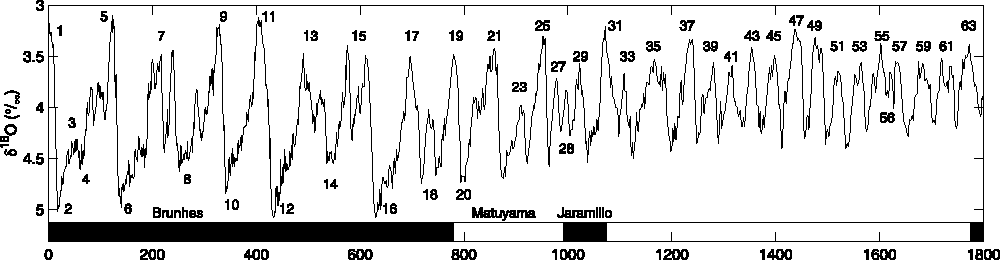
\includegraphics[width=80mm]{paleo-timeseries}
  \caption{Palaeo-climate records of the last 800\,ka.
           \textbf{(a)} Benthic oxygen isotope (\chem{\delta^{18}O}) record
           from a compilation of globally-distributed deep sea sediment cores
           \citep{Lisiecki.Raymo.2005}. Higher \chem{\delta^{18}O} values
           correspond to periods of lower temperatures \citep{Emiliani.1955}
           or lower global sea level, and thus higher ice volume stored in
           glaciers and ice sheets on land \citep{Shackleton.1967}.
           \textbf{(b)} Temperature anomalies ($\Delta T$) reconstructed from a
           central Antarctic ice core \citep[EPICA Dome~C,][]{Jouzel.etal.2007}.
           The grey bands indicate the approximate time span of the last
           glacial period of 110 to 10\,ka.}
  \label{fig:paleo-timeseries}
\end{figure}

\begin{figure}
  \centering
  \includegraphics[width=80mm]{paleo-glaciation}
  \caption{Spatial extent of ice sheet and glacier cover in the northern
           hemisphere \textbf{(a)} at present \citep{Patterson.Kelso.2014}, and
           \textbf{(b)} during the last glacial maximum
           \citep{Ehlers.Gibbard.2007}.}
  \label{fig:paleo-glaciation}
\end{figure}

% ======================================================================
\section{Field area description}
% ======================================================================

During the last glacial cycle, much of North America has been covered by ice.
At the last glacial maximum, apex of glaciation, three major ice sheets had
collided to form a continuous blanket of ice that spanned from Alaska to
Newfoundland, connecting with the Greenland ice sheet in the Canadian Arctic,
and extending as far south as Chicago and the Great Lakes
(\cref{fig:map-northamerica}). The Laurentide ice
sheet, largest of the three, was centred on the modern Hudson Bay,
and fully covered the Canadian Prairies, Eastern Canada, and the Great Lakes
Basin. The Innuitian ice sheet, much smaller, covered the northernmost Canadian
archipelago. Finally, the Cordilleran ice sheet capped the mountain ranges of
the Western Cordillera, which forms our region of focus in the present thesis.

\begin{figure}
  \centering
  \makebox[0pt]{\includegraphics{map-northamerica}}
  \caption{Relief map of northern North America showing a reconstruction of the
           areas covered by the Cordilleran (CIS), Laurentide (LIS), Innuitian
           (IIS) and Greenland (GIS) ice sheets during the last glacial maximum
           \citep[21.4 to 16.8\,cal\,\chem{^{14}C}\,kyr\,BP,][]{Dyke.2004}.
           The rectangular box delimits the model domain used in all simulation
           and most figures of this thesis. The background
           map consists of ETOPO1 \citep{Amante.Eakins.2009} and Natural Earth
           Data \citep{Patterson.Kelso.2014}.}
  \label{fig:map-northamerica}
\end{figure}

% ----------------------------------------------------------------------
\subsection{Topographic setting}
% ----------------------------------------------------------------------

The North American Cordillera forms a broad mountain system with an
average east-west width of about 1000\,km. Its topography is a complex
jigsaw of mountain ranges and interior basins (\cref{fig:map-cordillera}).
It was formed during multiple accretion phases associated with the closure of
several back-arc oceanic trenches over a 200\,Ma-long geological history
\citep{Sigloch.Mihalynuk.2013}.

Most of the dominant reliefs are found along two major ribbons that run
parallel to each other along the general orientation of the Cordillera
(\cref{fig:map-cordillera}). The western ribbon is formed by the Pacific Coast
orogenic belt. Major glaciated reliefs include,
from North to South, the Alaska Range, the Wrangell and Saint-Elias Mountains,
the Coast Mountains and the North Cascades. The eastern ribbon consists of the
Nevadan and Laramide belts, which are separated by the deep and strikingly
linear Rocky Mountain / Tintina Trench \mref. It includes the Selwyn and
MacKenzie Mountains in the north, and the Rocky Mountains in the South. The
Brooks Range, in northern Alaska, has been covered by ice, but its glaciers
were not connected to the main body of the Cordilleran ice sheet
\citep{Kaufman.Manley.2004}.

\todo{Go to geolibrary and check \emph{Geology of Canada} books and such for a
      reference about the three orogenic belts.}

The Cordillera comports several intermontane basins, which influenced the
patterns of ice flow. The two major depressions are the Fraser Plateau in
south-central British Columbia, and the Liard Lowland in northern British
Columbia. Between these two basins is found a mildly elevated, but extensive
and deeply incised mountain group, known as the Skeena Mountains.

The ubiquitously mountainous topography of the region presents a serious
obstacle to reconstructing past dynamics of the Cordilleran ice sheet. Because
of the irregular arrangement of valleys and ridges that formed the ice sheet's
floor, ice moved along tortuous and intertwined pathways, sometimes following
the major topographical troughs, and sometimes flowing across them
\citep{Davis.Mathews.1944, Kleman.etal.2010}. In terms of numerical glacier
modelling, this topography implies complex patterns of flow and stress
within the ice, and requires high-resolution, and thus, large computational
grids.

\begin{figure}
  \centering
  \makebox[0pt]{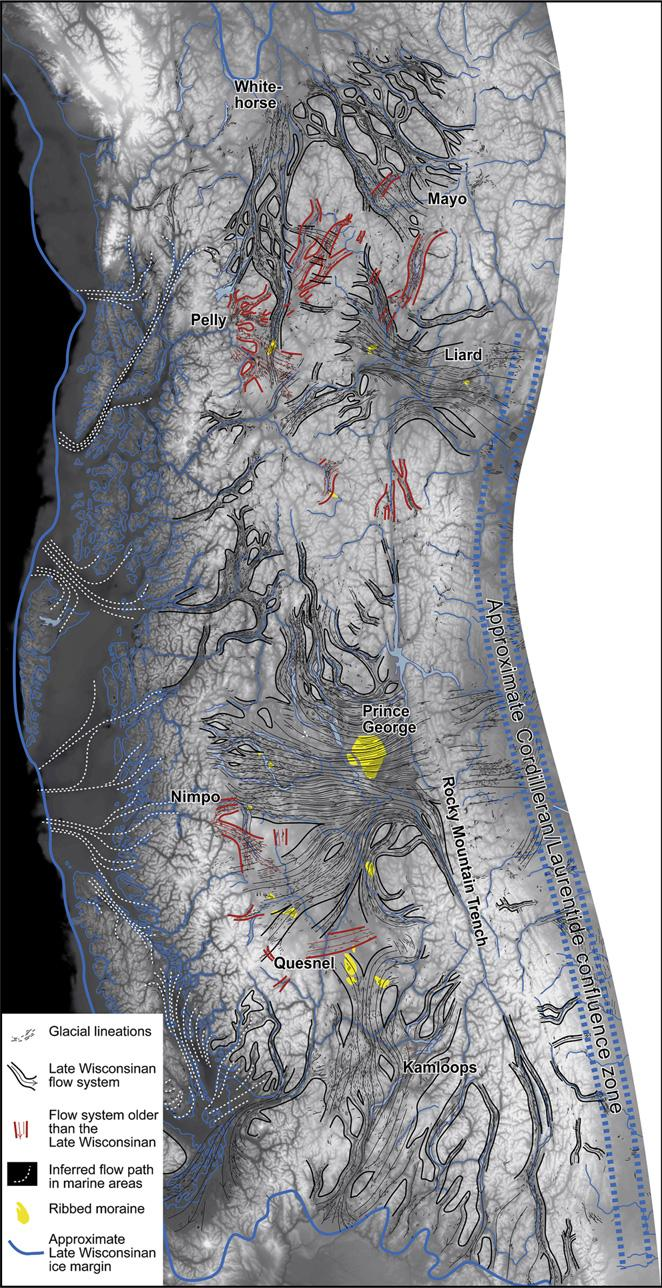
\includegraphics{map-cordillera}}
  \caption{Topographic map of the northern American Cordillera, oriented north.
           Cumulative last glacial maximum ice cover \citep{Dyke.2004} is
           marked in red, and the model domain in black.
           The background map consists of ETOPO1 \citep{Amante.Eakins.2009}
           and Natural Earth Data \citep{Patterson.Kelso.2014}.}
  \label{fig:map-cordillera}
\end{figure}

\begin{figure}
  \centering
  \makebox[0pt]{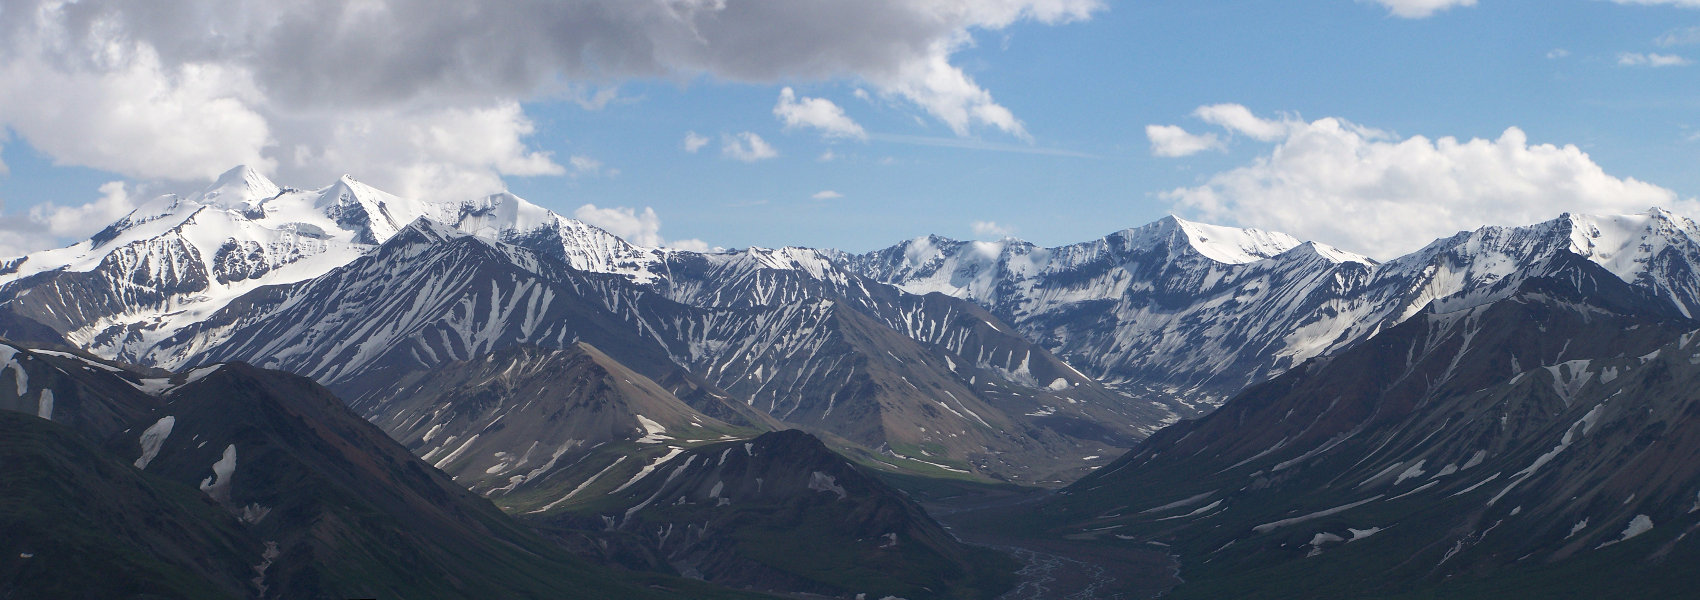
\includegraphics{photo-alaska-range}}
  \caption{The Alaska Range hosts several of the highest peaks in the North
           American Cordillera. Despite this fact and its northerly location,
           its north slope hosts relatively small glaciers only, which had not
           been much more extensive during the Last Glacial Maximum
           \citep{Kaufman.Manley.2004}, indicating dry climatic conditions.
           The Alaska Range is rapidly eroding, as shown by landslide-covered
           valley sides on this photograph.}
  \label{fig:photo-alaska-range}
\end{figure}

% ----------------------------------------------------------------------
\subsection{Climatic setting}
% ----------------------------------------------------------------------

The topographic complexity of the North American Cordillera is associated with
distinctive patterns of temperature and precipitation, whose effect is often
clearly visible in the landscape (\cref{fig:photo-fraser-valley}). Due to the
large latitudinal extent of the region, mean annual temperatures vary
significantly from north to south (\cref{fig:plot-atm}a). About half of the
model domain has mean annual temperature below freezing. However, seasonality,
here computed as the temperature difference between the warmest and the coldest
months, varies between around 10\,\degC\ along most of the Pacific Coast to
above 40\,\degC\ in the polar interior (\cref{fig:plot-atm}b). There exists a
partial correlation between cold regions and those that have a large
seasonality, so that many regions where mean annual temperature is well below
freezing point do experience warm summers.

Precipitation rates are highest on the western slopes of the Pacific Coast
ranges and decline quickly on the other side of the mountains
(\cref{fig:plot-atm}c). In terms of ice sheet mass balance, this contrast is
even reinforced by the difference in timing of the precipitation peak through
the year (\cref{fig:plot-atm}d). Coastal regions receive most precipitation
during winter and fall, thus as snow. On the contrary, many inland regions
experience dry winters, and most of the annual precipitation, there,
consequently falls
as rain during the ablation season. The climatic setting of the North American
Cordillera is described further in \CCLI, where its effects on the ice sheet
model response have been studied in detail.

\begin{figure}
  \centering
  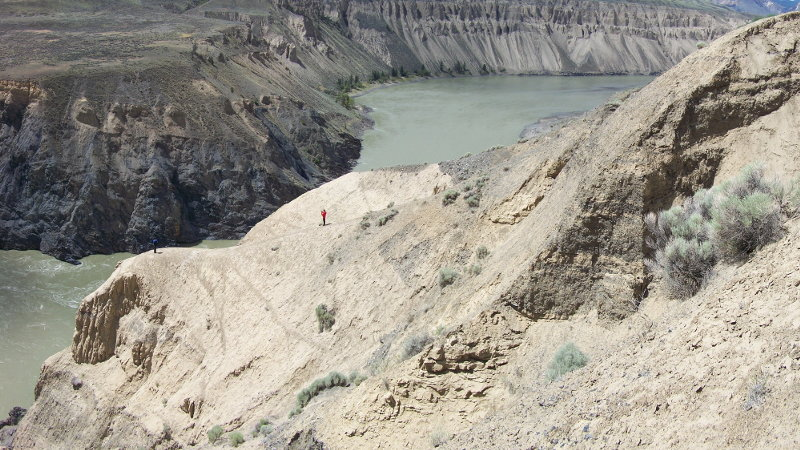
\includegraphics{photo-fraser-valley}
  \caption{This dry landscape of the Fraser Valley, central British Columbia,
           exhibits climatic contrasts at play in the Cordillera.}
  \label{fig:photo-fraser-valley}
\end{figure}

\begin{figure}
  \centering
  \makebox[0pt]{\includegraphics{plot-atm}}
  \caption{Some characteristics of the Cordilleran climate according to the
           North American Regional Reanalysis
           \citep[NARR,][]{Mesinger.etal.2006}}
  \label{fig:plot-atm}
\end{figure}


% ----------------------------------------------------------------------
\subsection{Glacial history}
% ----------------------------------------------------------------------

The first presence of an ice sheet in the Cordilleran mountains is indicated by
glaciofluvial deposits dated at $2.64^{+0.20}/_{-0.18}$\,Ma
\citep{Hidy.etal.2013}. This suggests that the North American Cordillera has
been glaciated many times, with the first glaciations occurring even before the
onset of the 100-ka glacial cycle (\cref{fig:paleo-timeseries}). However, only
the last few glaciations can be reconstructed from the geologic record, whereas
much of the older evidence has been overridden by subsequent glacial
re-advances and other geomorphological processes.

In the northern sector of the ice sheet, at least four glaciations have been
identified
    \citep{Duk-Rodkin.1999, Ward.etal.2007, Ward.etal.2008,
           Briner.Kaufman.2008, Demuro.etal.2012,
           Stroeven.etal.2010, Stroeven.etal.2014}.
The two older ones, often collectively referred to as the Reid glaciations,
pre-date the last glacial cycle, and thus are beyond the scope of this study.
The two younger glaciations, though, occurred both during the last glacial
cycle. First, the Gladstone glaciation reached its maximum between
$50.4\pm3.0$ and $54.3\pm2.0$\,\unit{^{10}Be\,ka} \citep{Ward.etal.2007},
during a period of high global ice volume on Earth, known as the Marine Isotope
Stage (MIS)~4. However, evidence from the Gladstone glaciation has not been
found in the southern part of the ice-covered region, making it difficult to
seize its magnitude. Second, the McConnell glaciation is associated with end
moraines of oldest minimum apparent exposure ages of
$15.7\pm1.5$ and $17.7\pm1.6$\,\unit{^{10}Be\,ka} \citep{Stroeven.etal.2014},
which corresponds to the last global ice volume maximum (MIS~2). In contrary to
the Gladstone glaciation, the McConnell glaciation has been correlated with a
contemporaneous advance of the southern ice sheet margin, known as the Fraser
glaciation, with a maximum extent framed between
$17.4$ and $16.4$\,\unit{^{14}C\,cal\,ka} \citep[Fig.~4]{Porter.Swanson.1998}.
Within errors inherent to the dating methods \citep{Heyman.etal.2011}, the
McConnell and Fraser glaciations correspond to the same glacial episode, which
resulted in the Last Glacial Maximum (LGM) extent of the Cordilleran ice sheet.
This is the period where most geological observations point at.

It is generally thought that the Cordilleran ice sheet was short-lived
    \citep[e.g.]{Clague.etal.1980, Clague.1985, Cosma.etal.2008}.
The ice sheet originated from the
coalescence of several mountain-centred ice caps \citep{Davis.Mathews.1944}.
During the last glacial maximum, ice covered most of the
Canadian Cordillera, and some of the adjacent land in north-western contiguous
USA and Alaska (\cref{fig:map-cordillera}).

The southern margin of the ice sheet has been studied extensively, and is in
several respects better understood than its northern counterpart
\citep{Booth.etal.2003}. It consists of different piedmont
lobes that have formed at the outlet of the main valleys. The Puget lobe
\citep[e.g.]{Thorson.1980, Porter.Swanson.1998} was the westernmost and
largest lobe. It covered the Puget Lowland, a region that currently includes
the cities of Vancouver and Seattle. East of the Cascade Range, were found the
Okanagan and Purcell lobes. The latter once dammed the Clark Fork River to form
Glacial Lake Missoula \citep{Pardee.1910}. As the ice sheet retreated, the lake
repeatedly and catastrophically drained to the Pacific Ocean
\citep{Bretz.1923,Waitt.1980}. These floods
contributed to shape a distinctive landscape, known as the Channeled Scabland.

The western margin of the ice sheet covered part of the continental shelf. An
ice cap covering Vancouver Island was well-connected to main body of ice on the
continent \mref. A significant part of the ice sheet thus drained into the Georgia
Strait and engulfed between Vancouver Island and the Olympic Peninsula where
it formed the Juan the Fuca marine ice lobe, calving into the Pacific Ocean \mref.
Further to the North, the ice margin reached Queen Charlotte Islands, yet the
archipelago may not have been fully covered by ice
flowing from the land. Submarine troughs likely indicate the erosional action of
former ice streams, yet it is not clear whether they have formed during the
last glacial cycle or earlier \mref.

Finally, the eastern margin of the ice sheet is the most unclear. Although it
is known that the Cordilleran ice sheet collided with its Laurentide neighbour,
the nature of the interaction between the two ice sheets and the precise
location of this junction is unclear, while little information exists on its
timing
    \citep[e.g.][]{Jackson.etal.1997, Bednarski.Smith.2007}.
Because the
present thesis focuses specifically on the Cordilleran ice sheet, our largest
assumption certainly consists of neglecting buttressing effects from the
Laurentide ice sheet.

The ice sheet is believed to have retreated quickly. Most of the evidence comes
from the Fraser Plateau, where it indicates that some of the highest relief
emerged from the ice prior to the lowlands, possibly resulting in thin,
stagnant ice remnants in the interior
    \citep{Fulton.1967, Fulton.1991, Margold.etal.2011, Margold.etal.2013a}.
Much less is known about ice sheet decay in the northern parts of the
ice-covered areas, but glacial landforms from the Liard Lowland suggest a
different mode of deglaciation, with active retreat of the ice lobe towards the
surrounding mountain ranges \citep{Margold.etal.2013}. Patterns of
deglaciation, as well as the possibility for a late-glacial re-advance, are
discussed in further detail and compared with modelling results in \CCYC.

% ======================================================================
\section{Numerical ice sheet model}
% ======================================================================

% ----------------------------------------------------------------------
\subsection{Overview}
% ----------------------------------------------------------------------

The simulations presented in this thesis use Parallel Ice Sheet Model (PISM),
an open-source, finite-difference, shallow ice-sheet model
\citep{PISM-authors.2014}. The model reads bedrock topography, sea level,
geothermal heat flux and climate forcing as inputs, and computes the thermal
and dynamic state of the ice sheet, and the associated thermal and
deformational response of an idealised lithosphere. The atmospheric and oceanic
envelopes are not part of the model. However, PISM includes boundary models
that provide simple parametrisations of their effect on the ice model at
supposedly well-defined interfaces (\cref{fig:model-interfaces}).

This section does not attempt to provide an extensive description of PISM,
which can be found in the on-line documentation \citep{PISM-authors.2014}.
Instead, it aims to highlight modelling choices made in the context of this
thesis, and give an overview of the physics involved in these choices.

\begin{figure}
  \centering
  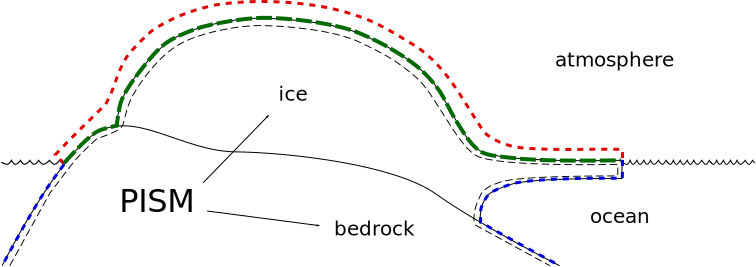
\includegraphics[width=80mm]{model-interfaces}
  \caption{Model interfaces in PISM. From \citet{PISM-authors.2014}.
           \todo{Redraw.}}
  \label{fig:model-interfaces}
\end{figure}

% ----------------------------------------------------------------------
\subsection{Field equations}
% ----------------------------------------------------------------------

\begin{figure}
  \centering
  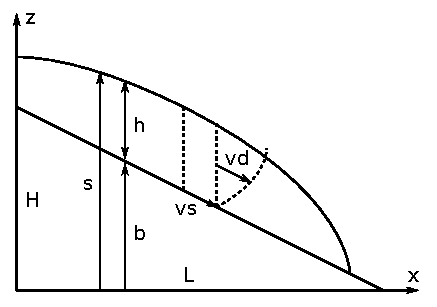
\includegraphics{model-variables}
  \caption{Sketch of notations used for the main variables of the ice sheet
           model.}
  \label{fig:model-variables}
\end{figure}

The thermodynamic core of the ice sheet model relies on four elementary field
equations. Firstly, ice flow is assumed \emph{incompressible}. Hence, the ice
density, $\rho$, is constant, and the
conservation of mass implies a conservation of volume, which can be expressed
in terms of the ice velocity vector, $\vv$, by
\begin{equation}
    \label{eqn:incompressibility}
    \div{\vv} = 0 \,.
\end{equation}

Secondly, the \emph{balance of stresses} is expressed by the Stokes equation,
thus assuming creeping flow. In other words, ice is considered as a slow-moving
fluid whose deformation is entirely controlled by internal friction, here
expressed by the Cauchy stress tensor, $\CST$, and gravity, $\vect{g}$:
\begin{equation}
    \label{eqn:stressbalance}
    \tdiv{\CST} + \rho\,\vect{g} = \vect{0} \,.
\end{equation}

Thirdly, after defining the strain-rate tensor
${\SRT = \frac{1}{2}(\tgrad{\vv} + \tgrad{\vv}^{\mathrm{T}})}$,
and the deviatoric stress tensor, ${\DST = \CST - p\,\IDT}$,
where $p=\frac{1}{3}\tr(\CST)$ is the hydrostatic pressure and
$\tens{\delta}$ is the identity tensor, a \emph{constitutive law} for ice based
on laboratory experiments is used to relate these two quantities. It reads:
\begin{equation}
    \label{eqn:glenslaw}
    \SRT = A\,\tau_e^{n-1}\,\DST \,.
\end{equation}
The equivalent stress, $\tau_e$, is defined by
${\tau_e}^2 = -\mathrm{II}_{\DST} = \frac{1}{2} \tr(\DST^2)$,
where $\mathrm{II}_{\DST}$ is the second invariant of the stress tensor.
The ice softness coefficient, $A$, depends on ice temperature, pressure, and
water content through an Arrhenius-type law,
\begin{equation}
    A =
    \begin{cases}
        A_c (1+f\omega)\,e^\frac{-Q_c}{RT_{pa}}
            & \text{if}\ T < T_c \,, \\
        A_w (1+f\omega)\,e^\frac{-Q_w}{RT_{pa}}
            & \text{if}\ T \ge T_c \,,
    \end{cases}
\end{equation}
where $T_{pa}$ is the pressure-adjusted temperature calculated using the
Clapeyron relation, ${T_{pa} = T - \beta p}$. The water fraction, $\omega$, is
capped at a threshold of 0.01, above which no measurements are available.

Letting ${\doteps_e}^2 = \frac{1}{2} \tr(\SRT^2)$ and $B=A^{-1/n}$, the
constitutive law (\ref{eqn:glenslaw}) can be rewritten using a sometimes more
convenient, inverted formulation,
\begin{equation}
    \label{eqn:invglenslaw}
    \DST = B\,\doteps_e^{1/n-1}\,\SRT \,.
\end{equation}
By analogy to Newtonian flow, an apparent viscosity, $\nu$, can then be defined
by $\DST = \nu\,\SRT$, thus yielding

\begin{equation}
    \label{eqn:viscosity}
    \nu = \frac{B}{2}\,\doteps_e^{1/n-1} \,.
\end{equation}

Finally, the evolution of temperature within the ice is governed by the
\emph{conservation of energy}. In PISM, the conservation of energy uses an
enthalpy formulation in order to account for thermodynamic effects associated
with internal phase changes in the glacier. This enthalpy ($H$) formulation
reads
\begin{equation}
    \label{eqn:enthalpy}
    \rho \left(\matdv{H}\right)
        = -\div{\vect{q}} + \frac{\nu\doteps_e^2}{4} \,,
\end{equation}
where $\vect{q}$ represents the heat flow and
${\frac{\nu\dot{\epsilon_e}^2}{4} = \tr(\DST\SRT)}$ is a
source term corresponding to strain heat release. In the case where ice
temperature, $T$, is below the pressure-melting point, the enthalpy can be
expressed as $H=c\,T$, while the heat flow is given by Fourier's law,
$\vect{q} = k\,\grad{T}$. Consequently, the enthalpy equation
(\ref{eqn:enthalpy}) can be rewritten using a more familiar, cold-ice,
temperature formulation,
\begin{equation}
    \label{eqn:temperature}
    \matdv{T} = \frac{k}{\rho c} \Delta T
                + \frac{\nu\doteps_e^2}{4\rho c} \,,
\end{equation}
where $c$ denotes the specific heat capacity of the ice and $k$ is its thermal
conductivity.

\Cref{eqn:incompressibility,eqn:stressbalance,eqn:glenslaw,eqn:enthalpy}
constitute the thermodynamic basis
of our model. However, their resolution in full form implies a computational
demand too high for multi-millennial, continental-scale applications, such as
the numerical modelling of the Cordilleran ice sheet through the last glacial
cycle, thus requiring shallow approximations.

\begin{table}
  \centering
  \caption{Constant parameters of the ice flow model.
           \todo{find a better reference than \citet{Aschwanden.etal.2012}
                 for all the physical constants. Double-check
                 \citet{Paterson.Budd.1982} and add missing references.}}
  \label{tab:iceflowparams}
  \makebox[0pt]{\begin{tabular*}{165mm}{@{\extracolsep{\fill}}rlrll}
    \hline
    Not.    & Name & Value & Unit & Source \\
    \hline

    $\rho$  & Ice density
            & 910
            & \unit{kg\,m^{-3}}
            & \citet{Aschwanden.etal.2012} \\

    $g$     & Standard gravity
            & 9.81
            & \unit{m\,s^{-2}}
            & \citet{Aschwanden.etal.2012} \\

    $n$     & Glen exponent
            & 3
            & -
            & \mref \\

    $A_c$   & Ice hardness coefficient cold
            & 3.61\e{-13}
            & \unit{Pa^{-3}\,s^{-1}}
            & \citet{Paterson.Budd.1982} \\

    $A_w$   & Ice hardness coefficient warm
            & 1.73\e3
            & \unit{Pa^{-3}\,s^{-1}}
            & \citet{Paterson.Budd.1982} \\

    $Q_c$   & Flow law activation energy cold
            & 6.0\e4
            & \unit{J\,mol^{-1}}
            & \citet{Paterson.Budd.1982} \\

    $Q_w$   & Flow law activation energy warm
            & 13.9\e4
            & \unit{J\,mol^{-1}}
            & \citet{Paterson.Budd.1982} \\

    $R$     & Ideal gas constant
            & 8.31441
            & \unit{J\,mol^{-1}\,K^{-1}}
            & \mref \\

    $T_c$   & Flow law critical temperature
            & 263.15
            & \unit{K}
            & \citet{Paterson.Budd.1982} \\

    $f$     & Flow law water fraction coeff.
            & 181.25
            & -
            & \citet{Lliboutry.Duval.1985} \\

    $\beta$ & Clapeyron constant
            & 7.9\e{-8}
            & \unit{K\,Pa^{-1}}
            & \citet{Luthi.etal.2002} \\

    $c_i$   & Ice specific heat capacity
            & 2009
            & \unit{J\,kg^{-1}\,K^{-1}}
            & \citet{Aschwanden.etal.2012} \\

    $c_w$   & Water specific heat capacity
            & 4170
            & \unit{J\,kg^{-1}\,K^{-1}}
            & \citet{Aschwanden.etal.2012} \\

    $k$     & Ice thermal conductivity
            & 2.10
            & \unit{J\,m^{-1}\,K^{-1}\,s^{-1}}
            & \citet{Aschwanden.etal.2012} \\

    $L$     & Water latent heat of fusion
            & 3.34\e5
            & \unit{J\,kg^{-1}\,K^{-1}}
            & \citet{Aschwanden.etal.2012} \\

    \hline
  \end{tabular*}}
\end{table}


% ----------------------------------------------------------------------
\subsection{Shallow approximations}
% ----------------------------------------------------------------------

PISM, the ice sheet model that we use, employ two well-documented
approximations of ice flow equations: the shallow ice approximation and the
the shallow shelf approximation. Although both approximations can be derived
from a rigorous scaling approach, we don't expand these lengthy derivations
here, assuming instead the simplifications and focusing on their effect.

\begin{figure}
  \centering
  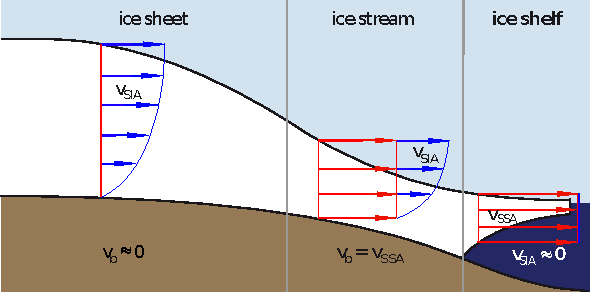
\includegraphics[width=80mm]{model-siassa}
  \caption{Shallow Ice Approximation (SIA) and Shallow Shelf Approximation
           (SSA) velocities in PISM. From \citet{Winkelmann.etal.2011}.
           \todo{Redraw.}}
  \label{fig:model-siassa}
\end{figure}


Distinguishing the hydrostatic and deviatoric components of the stress tensor,
the balance of stresses (\ref{eqn:stressbalance}) can be expanded into
\begin{equation}
    \tdiv{\DST} - \grad{p} + \rho\,\vect{g} = \vect{0} \,.
\end{equation}

Projecting along the three Cartesian coordinate axis, this reads
\begin{subequations}
\label{eqn:fullstokes}
\begin{align}
    \pdv{\tau_{xx}}{x} + \pdv{\tau_{xy}}{y} + \pdv{\tau_{xz}}{z}
        &= \pdv{p}{x} \,, \\
    \pdv{\tau_{yx}}{x} + \pdv{\tau_{yy}}{y} + \pdv{\tau_{yz}}{z}
        &= \pdv{p}{y} \,, \\
    \pdv{\tau_{zx}}{x} + \pdv{\tau_{zy}}{y} + \pdv{\tau_{zz}}{z}
        &= \pdv{p}{z} - \rho g \,.
\end{align}
\end{subequations}

The shallow ice approximation (SIA) assumes that basal friction is high enough
for the vertical shear stresses $\{\tau_{xz}, \tau_{yz}\}$ to predominate over
all other components of the deviatoric stress tensor. In this framework, the
projected stress-balance can be simplified to
\begin{subequations}
\label{eqn:sia}
\begin{align}
    \label{eqn:siax}
    \pdv{\tau_{xz}}{z} &= \pdv{p}{x} \,, \\
    \label{eqn:siay}
    \pdv{\tau_{yz}}{z} &= \pdv{p}{y} \,, \\
    \label{eqn:siaz}
    0 &= \pdv{p}{z} - \rho g \,.
\end{align}
\end{subequations}

Neglecting atmospheric pressure, \Cref{eqn:siaz} yield
\begin{equation}
    p = \rho g (s-z) \,,
\end{equation}
which can be re-introduced into \cref{eqn:siax,eqn:siay}, thus yielding the
expression of the horizontal shear stresses, sometimes referred to as driving
stresses,
\begin{subequations}
\begin{align}
    \tau_{xz} &= -\rho g (s-z) \pdv{s}{x} \,, \\
    \tau_{yz} &= -\rho g (s-z) \pdv{s}{x} \,.
\end{align}
\end{subequations}

Using the constitutive law (\ref{eqn:glenslaw}), vertical derivatives of
horizontal velocities can be related to the horizontal shear stresses:
\begin{subequations}
\begin{align}
    \pdv{v_x}{z} &= 2A (\tau_{xz}^2 + \tau_{yz}^2)^{n-1} \tau_{xz} \,, \\
    \pdv{v_y}{z} &= 2A (\tau_{xz}^2 + \tau_{yz}^2)^{n-1} \tau_{yz} \,.
\end{align}
\end{subequations}

Thus, within the framework of the SIA, horizontal velocities $\vv_{SIA}$ can be
directly expressed as a function of the slope gradient,
\begin{subequations}
\begin{align}
    \pdv{v_x}{z} &= -2A (\rho g)^n (s-z)^n
                    \left(\pdv{s}{x}+\pdv{s}{y}\right)^{n-1} \pdv{s}{x} \,, \\
    \pdv{v_y}{z} &= -2A (\rho g)^n (s-z)^n
                    \left(\pdv{s}{x}+\pdv{s}{y}\right)^{n-1} \pdv{s}{y} \,,
\end{align}
\end{subequations}
which yields, in vectorial notation,
\begin{equation}
    \label{eqn:vsia}
    \pdv{\vsia}{z} = -2A\,(\rho g)^n\,(s-z)^n\,|\grad{s}|^{n-1}\,\grad{s} \,.
\end{equation}

The shallow shelf approximation (SSA), on the opposite of the SIA, assumes that
basal friction is low enough for ice to deform predominantly by horizontal
expansion within the entire ice column. In this context, the stress-balance can
be simplified to
\begin{subequations}
\label{eqn:ssa}
\begin{align}
    \label{eqn:ssax}
    \pdv{\tau_{xx}}{x} + \pdv{\tau_{xy}}{y} + \pdv{\tau_{xz}}{z}
        &= \pdv{p}{x} \,, \\
    \label{eqn:ssay}
    \pdv{\tau_{yx}}{x} + \pdv{\tau_{yy}}{y} + \pdv{\tau_{yz}}{z}
        &= \pdv{p}{y} \,, \\
    \label{eqn:ssaz}
    \pdv{\tau_{zz}}{z} &= \pdv{p}{z} - \rho g \,,
\end{align}
\end{subequations}
and horizontal velocities can be assumed independent of depth, so that
\begin{align}
    \pdv{v_x}{z} &= 0 \,, \\
    \pdv{v_y}{z} &= 0 \,.
\end{align}

Once again neglecting atmospheric pressure, and remembering that $\tr(\DST)=0$,
\Cref{eqn:ssaz} yields
\begin{align}
    p &= \rho g (s-z) - \tau_{zz} \,, \\
      &= \rho g (s-z) + \tau_{xx} + \tau_{yy} \,,
\end{align}
which can be re-introduced into \cref{eqn:ssax,eqn:ssay}:
\begin{subequations}
\begin{align}
    2\pdv{\tau_{xx}}{x} - \pdv{\tau_{yy}}{x} + \pdv{\tau_{xy}}{y}
        + \pdv{\tau_{xz}}{z} &= \rho g \pdv{s}{x} \,, \\
    \pdv{\tau_{yx}}{x} + 2\pdv{\tau_{yy}}{y} - \pdv{\tau_{xx}}{y}
        + \pdv{\tau_{yz}}{z} &= \rho g \pdv{s}{y} \,.
\end{align}
\end{subequations}

Using the inverse formulation of the constitutive law \eqref{eqn:invglenslaw},
components of the deviatoric stress tensor can be replaced by corresponding
velocity components, yielding
\begin{subequations}
\begin{align}
    \pdv{x} \left[2\bar{\nu}
                  \left(2\pdv{v_x}{x} + \pdv{v_y}{y}\right) \right]
        + \pdv{y} \left[\bar{\nu}
                        \left(\pdv{v_x}{y} + \pdv{v_y}{x}\right) \right]
        + \pdv{\tau_{xz}}{z} &= \rho g \pdv{s}{x} \,, \\
    \pdv{x} \left[\bar{\nu}
                  \left(\pdv{v_x}{y} + \pdv{v_y}{x}\right) \right]
        + \pdv{y} \left[2\bar{\nu}
                        \left(\pdv{v_x}{x} + 2\pdv{v_y}{y}\right) \right]
         + \pdv{\tau_{yz}}{z} &= \rho g \pdv{s}{y} \,,
\end{align}
\end{subequations}
where $\bar{\nu}$ is the depth-integrated apparent viscosity defined by
\begin{equation}
    \bar{\nu} = \frac{1}{H}\int_b^s\nu \,.
\end{equation}

A final integration over the entire ice column yields
\begin{subequations}
\begin{align}
    \label{eqn:vssa}
    \pdv{x} \left[2\bar{\nu}h
                  \left(2\pdv{v_x}{x} + \pdv{v_y}{y}\right) \right]
        + \pdv{y} \left[\bar{\nu}h
                        \left(\pdv{v_x}{y} + \pdv{v_y}{x}\right) \right]
        + \tau_{bx} &= \rho gh \pdv{s}{x} \,, \\
    \pdv{x} \left[\bar{\nu}H
                  \left(\pdv{v_x}{y} + \pdv{v_y}{x}\right) \right]
        + \pdv{y} \left[2\bar{\nu}h
                        \left(\pdv{v_x}{x} + 2\pdv{v_y}{y}\right) \right]
        + \tau_{by} &= \rho gh \pdv{s}{y} \,,
\end{align}
\end{subequations}
where $\tau_{bx}$ and $\tau_{by}$ correspond to $x$ and $y$-components of the
basal traction, and will be determined by a sliding law.

In PISM, the SIA and SSA velocities are eventually added,
\begin{equation}
    \label{eqn:siassa}
    \vv = \vsia + \vssa \,.
\end{equation}
Because $\vsia$ is small where $\vssa$ is large and
reciprocally, we can expect the model to perform well in regions where
conditions for applicability of either the SIA or the SSA are met. However,
\cref{eqn:siassa} is a heuristic, and its validity in the zone of
transition between shear flow and longitudinal flow has not yet been
mathematically proven.


% ----------------------------------------------------------------------
\subsection{Basal sliding}
% ----------------------------------------------------------------------

Although the SIA is valid only under non-sliding conditions, the SSA requires
a sliding law as basal boundary condition, which in fact constitutes the main
control on SSA velocities and in turn locations of ice streams.

The simulations presented in this thesis use a pseudo-plastic sliding law,
\begin{equation}
    \label{eqn:pseudoplastic}
    \vect{\tau}_b = -\tau_c \frac{\vv_b}{{v_{th}}^q\,|\vv_b|^{1-q}} \,,
\end{equation}
where $\vect{\tau}_b$ is the basal traction force, $\vv_b$ is the basal
velocity, and $v_{th}$ is an arbitrary velocity threshold. In the case of
$q=0$, \cref{eqn:pseudoplastic} corresponds to a purely plastic law,
\begin{equation}
    \label{eqn:plastic}
    \vect{\tau}_b = -\tau_c \frac{\vv_b}{|\vv_b|} \,.
\end{equation}

However a non-zero exponent is chosen here in order to improve convergence. The
yield stress $\tau_c$ is related to till properties by the Mohr-Coulomb
criterion,
\begin{equation}
   \tau_c = c_0 + N\,\tan{\phi} \,.
\end{equation}

The till cohesion $c_0$ is assumed to be zero. The effective pressure on the
till, $N$, is determined by the modelled amount of water at the bed. However,
two different parametrisations are used within this thesis. In {\CCLI}, using
PISM~0.5, the effective pressure is linearly related to water content by a
simple parametrisation,
\begin{equation}
    N = \rho gh (1 - \alpha \frac{W}{W_{max}}) \,.
\end{equation}

In {\CCYC}, using PISM~0.6, the effective pressure is determined by an
empirical parametrisation based on laboratory experiments on Antarctic till,
\begin{equation}
    N = \delta \rho gh \, 10^{(e_0/C_c) (1 - (W/W_{max}))} \,.
\end{equation}

Drainage of water at the base of the ice sheet, although implemented in PISM,
is not included in simulations presented here for the sake of simplicity.
In turn, the amount of water at the bed, $W$, corresponds to the local
accumulation of basal melt-water. In varies from zero to $W_{max}$, a threshold
above which further melt exits the system.

Finally, the till friction angle $\phi$ is taken a~function of modern bed
elevation, with lowest values occurring at low elevations, thus accounting for
a weakening of till associated with the presence of marine sediments:
\begin{equation}
    \phi(x,y) =
    \begin{cases}
        \phi_0 & \text{if}\ b \le b_0 \,, \\
        \phi_0 + (\phi_1-\phi_0) \frac{b - b_0}{b_1-b_0}
                & \text{if}\ b_0 < b < b_1 \,, \\
        \phi_1 & \text{if}\ b_1 \le b \,,
    \end{cases}
\end{equation}
where $b_0=0$\,m is modern sea-level and $b_1=200$\,m is a rough average of
highest shoreline elevations in the model domain. The values of $\phi_1$ and
$\phi_2$ are chosen differently in \CCLI (10 and 30$^\circ$) and \CCYC
(15 and 45$^\circ$), but these choices are roughly equivalent in the case of a
saturated till ($W=W_{max}$).

\begin{table}
  \centering
  \caption{Constant parameters of the sliding model. Missing sources
           correspond to uncalibrated values.}
  \label{tab:slidingparams}
  \makebox[0pt]{\begin{tabular*}{165mm}{@{\extracolsep{\fill}}rlrll}
    \hline
    Not.    & Name & Value & Unit & Source \\
    \hline

    $q$     & Pseudo-plastic sliding exponent
            & 0.25
            & -
            & - \\

    $v_{th}$& Pseudo-plastic threshold velocity
            & 100.0
            & \unit{m\,yr^{-1}}
            & - \\

    $c_0$   & Till cohesion
            & 0.0
            & Pa
            & - \\

    $\alpha$& \todo{check value}
            & 0.95
            & -
            & - \\

    $\delta$& \todo{find a good name}
            & 0.02
            & -
            & - \\

    $e_0$   & Till reference void ratio
            & 0.69
            & -
            & \citet{Tulaczyk.etal.2000} \\

    $C_c$   & Till compressibility coefficient
            & 0.12
            & -
            & \citet{Tulaczyk.etal.2000} \\

    $W_{max}$ & Maximal till water thickness
            & 2.0
            & m
            & - \\

    $b_0$   & Altitude of max. friction angle
            & 0
            & m
            & - \\

    $b_1$   & Altitude of min. friction angle
            & 200
            & m
            & - \\

    $\phi_0$& Minimum friction angle
            & 10/15
            & \degree
            & - \\

    $\phi_1$& Maximum friction angle
            & 30/45
            & \degree
            & - \\

    \hline
  \end{tabular*}}
\end{table}


% ----------------------------------------------------------------------
\subsection{Bedrock response}
% ----------------------------------------------------------------------

The modelled ice sheet interacts with the underlying bedrock in two ways.
Firstly, bedrock temperatures are computed to a given depth by appending the
ice enthalpy model (\ref{eqn:enthalpy}) with an underlying bedrock thermal
model. The only process accounted for is heat conduction, hence this model
consists of a simple diffusion equation,
\begin{equation}
    \pdv{T}{t} = \frac{k_b}{\rho_b c_b} \Delta T \,,
\end{equation}
where $k_b$, $\rho_b$ and $c_b$ are the thermal conductivity, density and
specific heat capacity of the bedrock. Bedrock temperature is conditioned at
depth by a fixed upwards geothermal heat flux $q_G$. The bedrock thermal model
is necessary for modelling the Cordilleran ice sheet on multi-millennial
time-scales, because temperature fluctuations caused by climate change and
isolating effects of the ice sheet penetrate several hundred meters into the
rock, and eventually affect basal ice temperatures.

Secondly, bedrock elevation evolve in response to the ice load. The bedrock
deformation model used in this thesis describes the flexure of an elastic
lithosphere on top of an infinite half-space viscous mantle
\citep{Lingle.Clark.1985}. It can be described by a single differential
equation of the bed elevation, $b$,
\begin{equation}
    2\nu_m\,|\grad|\,\pdv{b}{t} + \rho_l g b + D\,\Delta^2 b = \sigma_{zzb} \,,
\end{equation}
where $\nu_m$ is mantle viscosity, $\rho_l$ is lithosphere density, $D$ is the
lithosphere's flexural rigidity, and $\sigma_{zzb}$ corresponds to the ice load
\citep{Bueler.etal.2007}. Here, $\Delta^2$ designs the biharmonic (Laplacian
square) operator of
linear elastic theory, while $|\grad|$ is a pseudo-differential operator
defined through the Fourier transform by \citet[Eq.~6]{Bueler.etal.2007}. In
the left-hand part of this equation, the first term accounts for mantle
relaxation, the second for point-wise isostasy, and the third for elastic
flexure. Due to high mantle viscosity, $\nu_m$, there exists a time lag between
the ice sheet growth and the isostatic bedrock response.
%$\nu=1\times10^{21}$\,Pa\,s
%$D=5\times10^{24}$\,N\,m
%$\rho_r = 3300$\,kg\,m$^{-3}$

\begin{table}
  \centering
  \caption{Constant parameters of the bedrock model.
           \todo{Find out what the bedrock density corresponds to. Track down
                 original sources in \citet{Ritz.1997}}}
  \label{tab:bedrockparams}
  \makebox[0pt]{\begin{tabular*}{165mm}{@{\extracolsep{\fill}}rlrll}
    \hline
    Not.    & Name & Value & Unit & Source \\
    \hline

    $\rho_b$& Bedrock density
            & 3300
            & \unit{kg\,m^{-3}}
            & \mref \\

    $c_b$   & Bedrock specific heat capacity
            & 1000
            & \unit{J\,kg^{-1}\,K^{-1}}
            & \citet{Ritz.1997} \\

    $k_b$   & Bedrock thermal conductivity
            & 3.0
            & \unit{J\,m^{-1}\,K^{-1}\,s^{-1}}
            & \citet{Ritz.1997} \\

    $\nu_m$ & Mantle viscosity
            & 1\e21
            & \unit{Pa\,s}
            & \citet{Lingle.Clark.1985} \\

    $\rho_l$& Lithosphere density
            & 3300
            & \unit{kg\,m^{-3}}
            & \citet{Lingle.Clark.1985} \\

    $D$     & Lithosphere flexural rigidity
            & 5.0\e24
            & \unit{N}
            & \citet{Lingle.Clark.1985} \\

    \hline
%	pism overrides:bootstrapping geothermal flux value no var = 0.070 ;
  \end{tabular*}}
\end{table}


% ----------------------------------------------------------------------
\subsection{Surface mass balance}
% ----------------------------------------------------------------------

At the interface between the ice sheet and the atmosphere (Fig.~??),
surfice mass fluxes are computed from monthly mean surface air temperature,
$T_m$, and monthly precipitation, $P_m$, by a temperature-index model
\citep[e.g.,][]{Hock.2003}. Surface accumulation, $a_s$, equals precipitation
when temperature is below ${T_0=0\,\degC}$, and decreases to zero linearly
with temperature between $T_0$ and ${T_1=2\,\degC}$,
\begin{equation}
    a_s =
    \begin{cases}
        0       & \text{if}\ T_m \le T_s \,, \\
        P_m \frac{T_m-T_s}{T_r-T_s}
                & \text{if}\ T_s < T_m < T_r \,, \\
        P_m     & \text{if}\ T_r \le T_m \,,
    \end{cases}
\end{equation}

Surface melt, $m_s$, is assumed proportional to the number of positive degree
days (PDD), defined over an arbitrary time interval, $[t_1, t_2]$, as the
integral of positive Celcius temperature $T-T_0$,
\begin{equation}
    \mathrm{PDD} = \int_{0}^{A}\max(T(t)-T_0,0)\,dt \,.
\end{equation}

For multimillenial simulations of palaeo-ice sheet evolution such as the ones
presented in this thesis, daily or hourly temperature data is not available,
forcing the PDD computation to rely on an idealised representation of the
annual temperature cycle $T_{ac}$. Sub-annual temperature variability around
the freezing point, however, significantly affects surface melt on a multi-year
scale \citep{Arnold.Mackay.1964}. It is then typically included in the models
under an assumption of normal temperature distribution, using a standard
deviation parameter $\sPDD$ in the PDD computation \citep{Braithwaite.1984},
PDDs can then be computed using a double-integral formulation
\citep{Reeh.1991},
\begin{equation}
    \PDD = \frac{1}{\sPDD\sqrt{2\pi}}
        \int_{t_1}^{t_2} \mathrm{d}t
        \int_{0}^{\infty} \mathrm{d}T \,
        T \exp\left({-\frac{(T-T_{ac})^2}{2\sPDD^2}}\right) \,,
\end{equation}
or more efficiently using an error function formulation
\citep{Calov.Greve.2005},
\begin{equation}
    \label{eqn:calovgreve}
    \PDD = \int_{t_1}^{t_2} \mathrm{d}t
        \left[\frac{\sPDD}{\sqrt{2\pi}}
                \exp\left({-\frac{T_{ac}^2}{2\sPDD^2}}\right)
              + \frac{T_{ac}}{2} \, \mathrm{erfc}
                \left(-\frac{T_{ac}}{\sqrt{2}\sPDD}\right)\right] \,.
\end{equation}

In the simulations presented here, \cref{eqn:calovgreve} is numerically
approximated using week-long sub-intervals. For each sub-interval, surface melt
is computed from PDDs and the available snow and ice depths using an algorithm
documented in the on-line documentation of PISM \citep{PISM-authors.2014}. This
algorythms employ different melt factors for snow ($F_s$) and for ice ($F_i$),
as derived from mass-balance measurements on contemporary glaciers in the
Coast and Rocky Mountains of British Columbia \citep{Shea.etal.2009}. In
{\CCLI}, the temperature standard deviation $\sPDD$ is a constant model
parameter. In {\CCYC}, it is computed from daily temperature values from the
North American Regional Reanalysis \citep[NARR,][]{Mesinger.etal.2006}, using
a method initially developed in {\PSDV}, and further improved in {\PSDP}.
%3.04\,\unit{mm\,{\degree}C^{-1}\,day^{-1}} for snow and
%4.59\,\unit{mm\,{\degree}C^{-1}\,day^{-1}} for ice

\begin{figure}
  \centering
  \includegraphics[width=80mm]{model-pdd}
  \caption{PDD model. From \citet{PISM-authors.2014} \todo{Redraw.}}
  \label{fig:model-pdd}
\end{figure}

\begin{table}
  \centering
  \caption{Constant parameters of the surface and atmosphere models.
           \todo{Find a reference for the snow and rain temperature thresholds,
                 maybe \citet{Hock.2003}.}}
  \label{tab:surfaceparams}
  \makebox[0pt]{\begin{tabular*}{165mm}{@{\extracolsep{\fill}}rlrll}
    \hline
    Not.    & Name & Value & Unit & Source \\
    \hline

    $T_s$   & Temperature of snow precipitation
            & 273.15
            & \unit{K}
            & \mref \\

    $T_r$   & Temperature of rain precipitation
            & 275.15
            & \unit{K}
            & \mref \\

    $F_s$   & Degree-day factor for ice
            & 3.04\e{-3}
            & \unit{m\,K^{-1}\,day^{-1}}
            & \citet{Shea.etal.2009} \\

    $F_i$   & Degree-day factor for ice
            & 4.59\e{-3}
            & \unit{m\,K^{-1}\,day^{-1}}
            & \citet{Shea.etal.2009} \\

    $\gamma$& Air temperature lapse-rate
            & 6\e{-3}
            & \unit{K\,m{-1}}
            & - \\

    \hline
  \end{tabular*}}
\end{table}


% ----------------------------------------------------------------------
\subsection{Atmospheric forcing}
% ----------------------------------------------------------------------

Atmospheric forcing of the model consists of a present-day monthly climatology,
$\{T_{m0}, P_{m0}\}$, modified by a lapse-rate correction, ${\Delta}T_{LR}$,
and a temperature-offset correction, ${\Delta}T_{TS}$,
\begin{subequations}
\begin{align}
    T_m(t, x, y) &= T_{m0}(x, y) + {\Delta}T_{LR}(t)
                                 + {\Delta}T_{TS}(t, x, y) \,, \\
    P_m(t, x, y) &= P_{m0}(x, y) \,.
\end{align}
\end{subequations}

\todo{Figure. Boundary models data flow chart}

The present-day climatology, $\{T_{m0}, P_{m0}\}$, is computed from
near-surface air temperature and precipitation rate fields extracted from
observational data and atmospheric reanalyses.
The lapse-rate correction, ${\Delta}T_{LR}$, is computed in relation to the
climate input reference bedrock topography, $b_{ref}$,
\begin{align}
    {\Delta}T_{LR}(t, x, y) &= -\gamma [s(t, x, y)-b_{ref}(x, y)] \\
                            &= -\gamma [h(t, x, y)+b(t, x, y)-b_{ref}(x, y)]\,,
\end{align}
thus accounting for the evolution of ice thickness, $h$, on the one hand, and
for differences between the the ice flow model basal topography, $b$, and the
climate input topography, $b_{ref}$, on the other hand. All simulations use an
annual temperature lapse rate of $\gamma = 6\,\unit{\degC\,km^{-1}}$.

\CCLI tests the sensitivity of the model to different input present-day
climatologies, $\{T_{m0}, P_{m0}\}$, while the temperature-offset corrections,
${\Delta}T_{TS}$, uses constant values ranging from -10 to 0\,\degC. \CCYC,
on the opposite, tests model sensitivity to time-dependent temperature-offset
corrections derived from different palaeo-temperature proxy records.

\begin{table}
  \centering
  \caption{Sources of forcing data used to inform the ice sheet model.}
  \label{tab:datasources}
  \makebox[0pt]{\begin{tabular*}{160mm}{@{\extracolsep{\fill}}llll}
    \hline
    Name        & Type & Original reference & Employed in \\
    \hline

    ETOPO1      & Bedrock topography
                & \citet{Amante.Eakins.2009}
                & \CCLI, \CCYC \\

    WorldClim   & Gridded observations
                & \citet{Hijmans.etal.2005}
                & \CCLI \\

    NCEP/NCAR   & Atmospheric reanalysis
                & \citet{Kalnay.etal.1996}
                & \CCLI \\

    ERA-40      & \qquad '' \qquad
                & \citet{Uppala.etal.2005}
                & \PSDP \\

    ERA-Interim & \qquad '' \qquad
                & \citet{Dee.etal.2011}
                & \CCLI, \PSDV \\

    CFSR        & \qquad '' \qquad
                & \citet{Saha.etal.2010}
                & \CCLI \\

    NARR        & \qquad '' \qquad
                & \citet{Mesinger.etal.2006}
                & \CCLI, \CCYC \\

    GRIP        & Ice-core \chem{\delta^{18}O} record
                & \citet{Dansgaard.etal.1993}
                & \CCYC \\

    NGRIP       & \qquad '' \qquad
                & \citet{Andersen.etal.2004}
                & \CCYC \\

    EPICA       & \qquad '' \qquad
                & \citet{Jouzel.etal.2007}
                & \CCYC \\

    Vostok      & \qquad '' \qquad
                & \citet{Petit.etal.1999}
                & \CCYC \\

    ODP~1012    & Sea-floor \chem{U^{K'}_{37}} record
                & \citet{Herbert.etal.2001}
                & \CCYC \\

    ODP~1020    & \qquad '' \qquad
                & \citet{Herbert.etal.2001}
                & \CCYC \\

    \hline
  \end{tabular*}}
\end{table}


% ----------------------------------------------------------------------
\subsection{Numerical implementation}
% ----------------------------------------------------------------------

\begin{table}
  \centering
  \caption{Properties of the Canadian Atlas Lambert conformal conic projection
           (EPSG code~3978) and the GRS~1980 ellipsoid, and corresponding
           PROJ.4 parameter names, as used in all model runs, ice volume and
           area calculations, and most figures.}
  \label{tab:projparams}
  \makebox[0pt]{\begin{tabular*}{80mm}{@{\extracolsep{\fill}}lcc}
    \hline
    Parameter               & Name              & Value \\
    \hline
    Projection name         & \texttt{+proj}    & \texttt{lcc} \\
    Central meridian        & \texttt{+lon\_0}  & 95\degree W \\
    Latitude of origin      & \texttt{+lat\_0}  & 49\degree N \\
    First secant parallel   & \texttt{+lat\_1}  & 49\degree N \\
    Second secant parallel  & \texttt{+lat\_2}  & 77\degree N \\
    Semimajor radius        & \texttt{+a}       & 6378137\,m \\
    Reciprocal flattening   & \texttt{+rf}      & 298.257222101 \\
    \hline
  \end{tabular*}}
\end{table}

% ======================================================================
\section{Software tools and contributions}
% ======================================================================

% ----------------------------------------------------------------------
\subsection{Computational workflow}
% ----------------------------------------------------------------------
\todo{Figure. computational workflow}

% ----------------------------------------------------------------------
\subsection{A Python PDD model}
% ----------------------------------------------------------------------
\todo{Figure. PyPDD demo example}

% ----------------------------------------------------------------------
\subsection{Pre-processing scripts for GRASS GIS}
% ----------------------------------------------------------------------

% ----------------------------------------------------------------------
\subsection{Plotting tools for PISM}
% ----------------------------------------------------------------------
\todo{Figure. Plotting tools example}

% ----------------------------------------------------------------------
\subsection{Contributions to PISM}
% ----------------------------------------------------------------------
\todo{Table. PISM ``issues'' identified}

% ======================================================================
\section{Results summary}
% ======================================================================

% ----------------------------------------------------------------------
\subsection{Constant-climate runs}
% ----------------------------------------------------------------------
\todo{Figure. 3km last glacial maximum poster run?}

% ----------------------------------------------------------------------
\subsection{Daily temperature variability}
% ----------------------------------------------------------------------
\todo{Figure. Sigma distribution map}\\
\todo{Figure. Sigma effect on Cordillera runs}

% ----------------------------------------------------------------------
\subsection{Transient-climate runs}
% ----------------------------------------------------------------------
\todo{Figure. Deglaciation streamplot}\\
\todo{Figure. Cumulative ice displacement map}

% ======================================================================
\section{Future perpectives}
% ======================================================================
% Model improvements
% Fieldwork
% Geomorphological-oriented plots

\begin{figure}
  \centering
  \makebox[0pt]{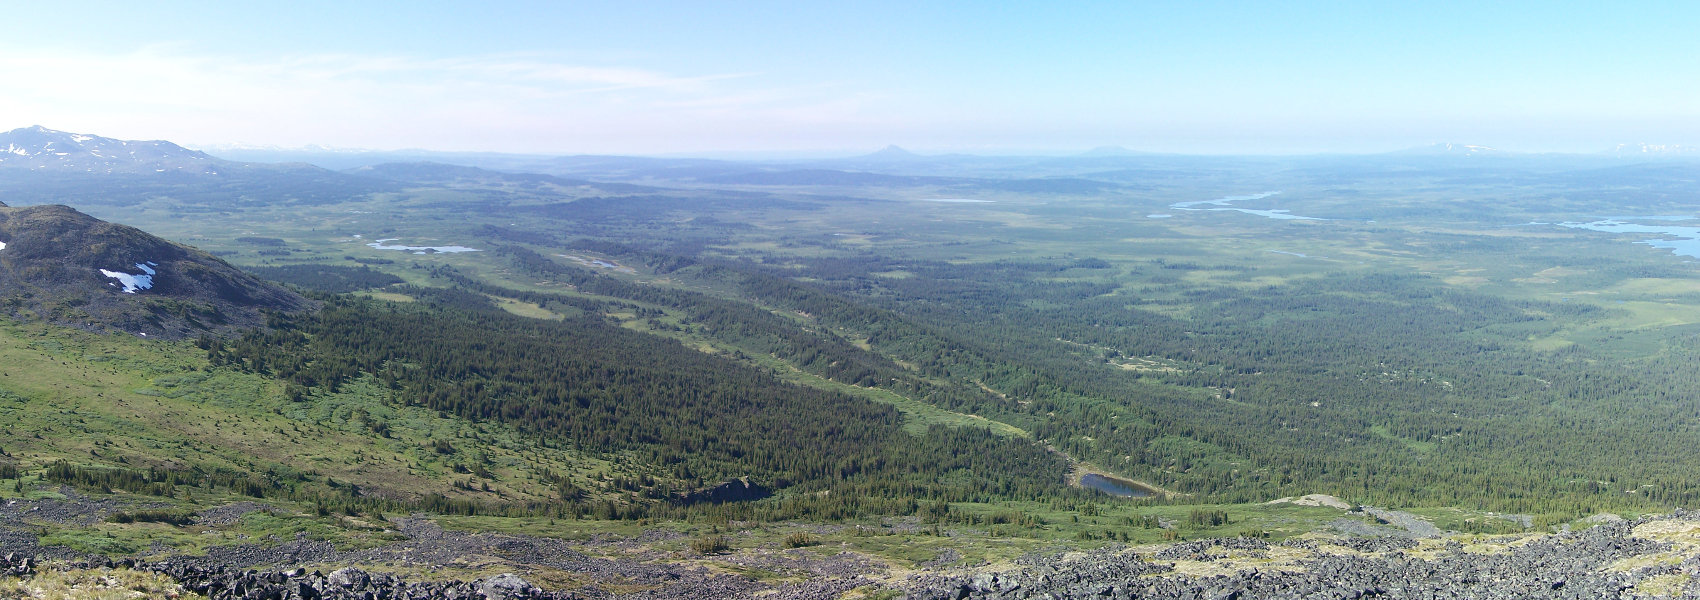
\includegraphics{photo-tuya-moraine}}
  \caption{The Tuya Lake Moraine in northern British Columbia.}
  \label{fig:photo-tuya-moraine}
\end{figure}

% References
\newcommand{\urlprefix}[0]{}  % remove default "URL" prefix
\bibliographystyle{copernicus}
\bibliography{refs/references.bib}

% ----------------------------------------------------------------------
\end{document}
% ----------------------------------------------------------------------
